\section{Auswertung}
\label{sec:Auswertung}

\subsection{Bestimmung von RC über Entladung}
\label{sec:auswertung1}
Die Messwerte aus der ersten Messreihe, \ref{sec:messung1},
werden nach \eqref{eqn:aformel} umgerechnet. In Abbildung \ref{fig:linregA} sind
die Werte aufgetragen. Die Ausgleichsgerade bestimmt sich zu
\begin{equation}
  y = mt+b = (\num{-13.05(07)})\frac{1}{\symup{s}}\:t + (\num{0.014(009)}).
\end{equation}
Wobei $m = - \sfrac{1}{\text{RC}}$ gilt und die erweiterte Zeitkonstante somit
\begin{equation*}
  \left(\left(\symup{R_g + R}\right)\symup{C}\right)_1 = \SI{0.0766(0004)}{\second}
\end{equation*}
ist. Das folgt aus dem Aufbau \ref{fig:aufbau1}, wobei
$\symup{R}_\text{g} = \SI{650}{\ohm}$, \ref{eqn:widerstandgenerator},
der Gesamtwiderstand des Funktionsgenerators ist.
\begin{figure}
  \centering
  \includegraphics[width=\textwidth]{build/linreg_a.pdf}
  \caption{Messwerte der Entladung und Ausgleichsgerade.}
  \label{fig:linregA}
\end{figure}

\begin{table}
  \centering
  \caption{Messwerte der Entladung.}
  \label{tab:messwerteA}
  \begin{tabular}{
    S[table-format=3.0]
    S[table-format=2.2]
    S[table-format=1.2]
    }
    \toprule
    {$t \: [\si{\milli\second}]$}
    & {$U_\text{C} \: [\si{\volt}]$}
    &{$\log\!\left(\frac{U_\text{C}}{U_0}\right)$}
    \\
    \midrule
       0 & 18.4  &  0    \\
      20 & 14.6  & -0.23 \\
      40 & 11.2  & -0.50 \\
      60 &  8.48 & -0.77 \\
      80 &  6.56 & -1.03 \\
     100 &  5.04 & -1.29 \\
     120 &  3.92 & -1.55 \\
     140 &  2.94 & -1.83 \\
     160 &  2.34 & -2.06 \\
     180 &  1.74 & -2.36 \\
     200 &  1.40 & -2.58 \\
    \bottomrule
  \end{tabular}
\end{table}

\begin{figure}
  \centering
  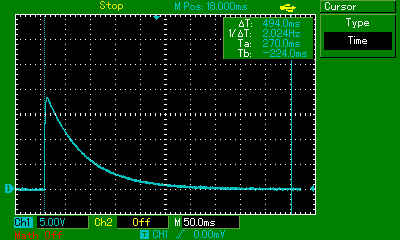
\includegraphics{content/Bilder/entladevorgang.jpg}
  \caption{Entladevorgang}
  \label{fig:entladung}
\end{figure}

\newpage

\subsection{Bestimmung von RC über die frequenzabhängige Amplitude}
\label{sec:auswertung2}
Die Messwerte, zur Bestimmung der Frequenzabhängigkeit der Phase, aus der
zweiten Messreihe, \eqref{sec:messung2}, werden mittels
\eqref{eqn:bformel} nach $\frac{U_\text{C}}{U_\text{C}(0)}$ umgestellt und gegen die Frequenz
aufgetragen. In Abbildung \eqref{fig:freqAmp} sind die Werte aufgetragen.

Der zweite Wert mit f = $30 \:\sfrac{1}{\symup{s}}$ wurde, nach Absprache,
für die Auswertung ausgelassen, da er sehr aus dem Schema fällt.
\\
Für Frequenzen, die klein gegen $1 / \symup{RC}$ sind, verhält sich $U(t)$ wie
$U_\text{C}(t)$. Es bildet sich eine
Phasenverschiebung zwischen Generator- und Kondensatorspannung aus, was in
einem Abfallen der Kondensatorspannung resultiert, wie der Abbildung
\eqref{fig:freqAmp} entnommen werden kann.
Daraus bestätigt sich, dass RC-Glieder auch als Tiefpässe benutzt werden können.
Tiefpässe lassen Frequenzen die klein gegen $1 / \symup{RC}$ nahezu ungehindert
durch und unterdrücken große Frequenzen.

Der Fit, nach Gleichung \ref{eqn:bformel}, ergibt
\begin{equation*}
  (\symup{RC})_2 = \SI{1.365(0019)e-3}{\second}.
\end{equation*}

\begin{figure}
  \includegraphics[width=\textwidth]{build/amplitudenplot.pdf}
  \caption{Frequenzabhängigkeit der Kondensatorspannungs-Amplitude.}
  \label{fig:freqAmp}
\end{figure}

\begin{table}
  \centering
  \caption{Werte für die Amplitudenabhängigkeit von Frequenz \ref{fig:freqAmp} und Phase \ref{fig:phase}.}
  \label{tab:messwerteB}
  \begin{tabular}{
    S[table-format=4.0]
    |S[table-format=2.1]
    S[table-format=2.2]
    S[table-format=1.3]
    |S[table-format=4.2]
    S[table-format=2.3]
    }
    \toprule
    {$f \: [\si{\per\second}]$}
    & {$U_0 \: [\si{\volt}]$}
    & {$U_\text{C} \: [\si{\volt}]$}
    & {$\frac{U_\text{C}}{U_\text{C}(0)}$}
    & {$t \: [\si{\micro\second}]$}
    & {$\phi \: [\si{\degree}]$}
    \\
    \midrule
      10 &  19.4 & 18.50 & 1.000 & 2000.00 & 7.2    \\
      30 &  19.4 & 18.30 &       &  960.00 & 10.368 \\
      70 &  19.4 & 16.24 & 0.878 & 1240.00 & 31.248 \\
     100 &  19.3 & 13.97 & 0.755 & 1160.00 & 41.76  \\
     300 &  19.3 &  6.57 & 0.355 &  640.00 & 69.12  \\
     700 &  19.2 &  2.95 & 0.159 &  320.00 & 80.64  \\
    1000 &  19.2 &  2.09 & 0.113 &  232.00 & 83.52  \\
    2000 &  19.2 &  1.05 & 0.057 &  122.00 & 87.84  \\
    3000 &  19.2 &  0.70 & 0.038 &   81.60 & 88.128 \\
    4000 &  19.2 &  0.53 & 0.029 &   62.40 & 89.856 \\
    5000 &  19.2 &  0.42 & 0.023 &   49.60 & 89.28  \\
    \bottomrule
  \end{tabular}
\end{table}
\newpage

\subsection{Phasenabhängigkeit der Kondensatorspannungs-Amplitude}
\label{sec:auswertung3}
Für die Meswerte der dritten Messreihe bestimmt man mittels Formel
\eqref{eqn:cformel} die Phasenverschiebung bei variabler Frequenz.
Die Phase $φ$ wird nach
\begin{align}
  φ &= 360 t f \cdot \num{1e-12}
  \intertext{für Grad und}
  φ &= 2 π t f \cdot \num{1e-12}
\end{align}
für Radiant bestimmt.
Die Phasenverschiebung ist in Abbildung \eqref{fig:phase} gegen die Frequenz
aufgetragen.
Die Zeitkonstante $\symup{RC}$ berechnet sich daraus zu
\begin{equation*}
  \symup{(RC)}_3 = \SI{1.412(0031)e-3}{\second}
\end{equation*}
\begin{figure}
  \includegraphics[width=\textwidth]{build/phasenplot.pdf}
  \caption{Phasenabhängigkeit der Kondensatorspannungs-Amplitude.}
  \label{fig:phase}
\end{figure}
Für den Plot \eqref{fig:polar} wird Gleichung \eqref{eqn:bformel} nach
$\frac{U_\text{C}}{U_\text{C}(0)}$ aufgelöst und gegen die Phase $φ$ aufgetragen.
Hierbei wurde die zuvor bestimmte Zeitkonstante $\symup{(RC)}_3$
benutzt.
\begin{figure}
  \centering
  \includegraphics[width=\textwidth]{build/polarplot.pdf}
  \caption{Polarplot der Phase gegen die reduzierte Amplitude.}
  \label{fig:polar}
\end{figure}

\newpage

\subsection{Zeitkonstante RC}

In der folgenden Tabelle sind noch einmal alle Werte der Zeitkonstanten
aufgelistet.

\begin{table}
  \centering
  \caption{Zeitkonstanten der Messreihen.}
  \label{tab:rc}
  \begin{tabular}{c c}
    \toprule
    {Auswertungsteil} & {$\symup{RC} \:/\:\si{\milli\second}$}
    \\
    \midrule
    5.1 & \num{7.66(04)}   \\
    5.2 & \num{1.365(0019)} \\
    5.3 & \num{1.412(0031)} \\
    \bottomrule
  \end{tabular}
\end{table}

Eine der Fehlerquellen, die hier nicht betrachtet wurden, ist der
Gesamtwiderstand von $\SI{650}{\ohm}$ der Spannungsquelle. Dieser wirkt sich nur
auf den RC-Wert aus \ref{sec:auswertung1} aus.
Der Mittelwert der beiden anderen Zeitkonstanten ist, nach \ref{eqn:mittelwert},
$(\text{RC})_M = \SI{1.3885e-3}{\second}$. Daraus ergibt sich,
\begin{equation*}
  \symup{R_g C} = \SI{7.52115e-3}{\second}
\end{equation*}
und
\begin{align}
  \symup{C}  &= \SI{115.7}{\micro\farad} \\
  \symup{R}  &= \SI{12}{\ohm}.
  \label{eqn:rcendlich}
\end{align}

\newpage

\subsection{Integratorfunktion des RC-Schwingkreises}
\label{sec:auswertung4}

An den zu integrierenden Funktionen auf Kanal 2 sieht man sehr gut die Integratorfunkion des RC-Kreises.
Die Rechteckspannung wird, nach der Integration, an ihren Extrema zu Geraden.
Das heißt sie wird zu einer Dreiecksspannung. Die Sinusfunktion wird zum Cosinus
und die Dreieckspannung wird integriert zu einer Art phasenverschobenen
Sinusfunktion.
\begin{figure}
  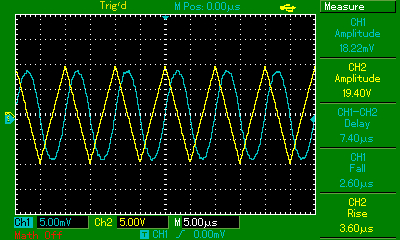
\includegraphics{content/Bilder/dreieck_integral.jpg}
  \caption{Integration für Dreieckspannung}
  \label{fig:deieckint}
\end{figure}

\begin{figure}
  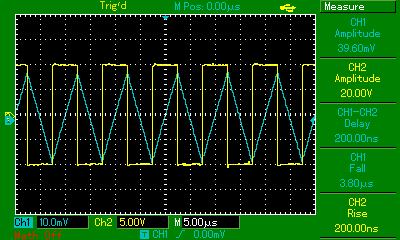
\includegraphics{content/Bilder/rechteck_integral.jpg}
  \caption{Integration für Rechteckspannung}
  \label{fig:rechteckint}
\end{figure}

\begin{figure}
  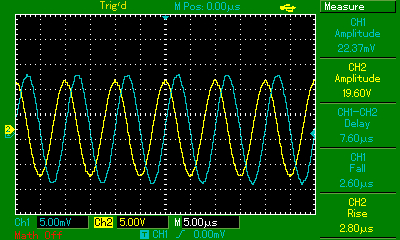
\includegraphics{content/Bilder/sinus_integral.jpg}
  \caption{Integration für Sinusspannung}
  \label{fig:sinusint}
\end{figure}
